\documentclass{article}

\usepackage[T1]{fontenc}    %Schriftart des Dokumentes
\usepackage[british]{babel} %Dokumentensprache, hier Deutsch
\usepackage{amsmath, amssymb, stmaryrd} %mathematische Schriftzeichen
\usepackage{graphicx} %Einfügen von Grafiken
\usepackage{wrapfig}
\usepackage{bm}

\setlength{\parindent}{0pt} %Einrückung von Absätzen auf null gesetzt
\setlength{\parskip}{10pt} %Abstand zischen Absätzen auf 10pt gesetzt

\title{Experiment 41: Temperature measurement}
\author{Matthias Kuntz}
\date{13.09.2023}

\begin{document}

\maketitle

%-------------------------EINLEITUNG-------------------------
\section{Introduction}

\subsection{Basics}

\subsection{Experiment Setup}

%---------------VERSUCHSPROTOKOLL MIT MESSDATEN---------------
\newpage

\section{Measurement Protocol}

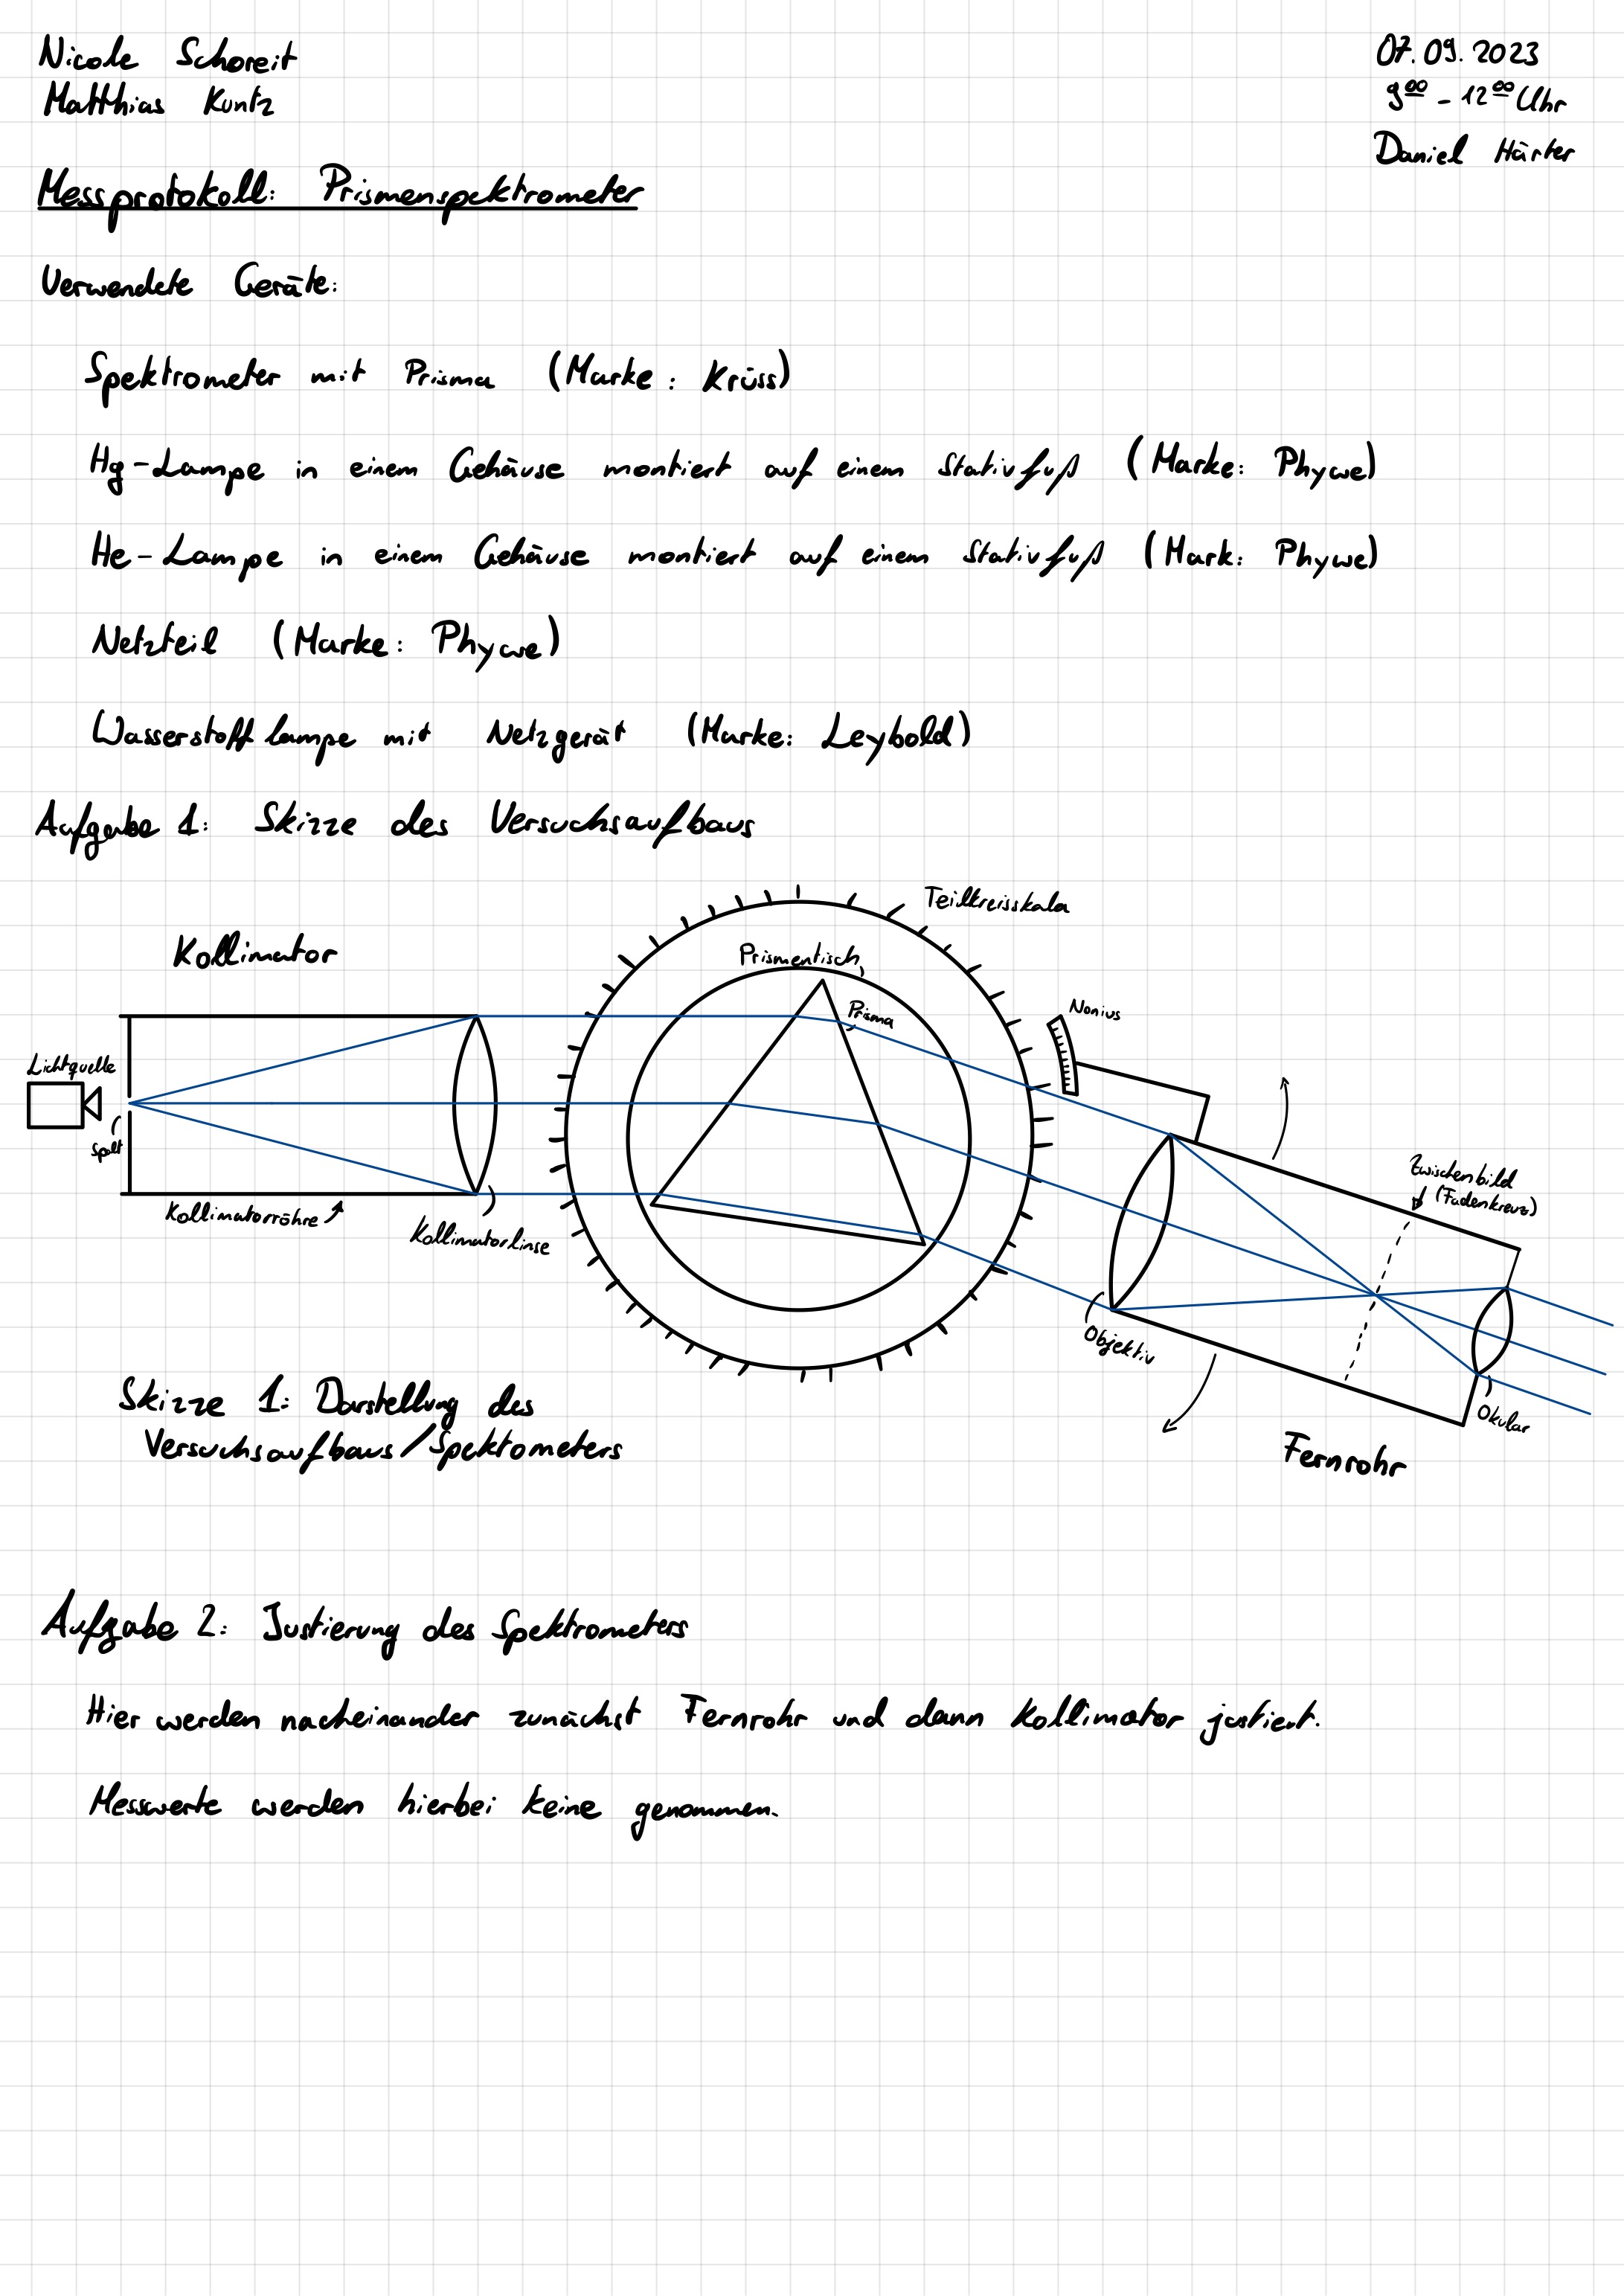
\includegraphics[width=\textwidth]{graphics/mess1.jpg}
\newpage
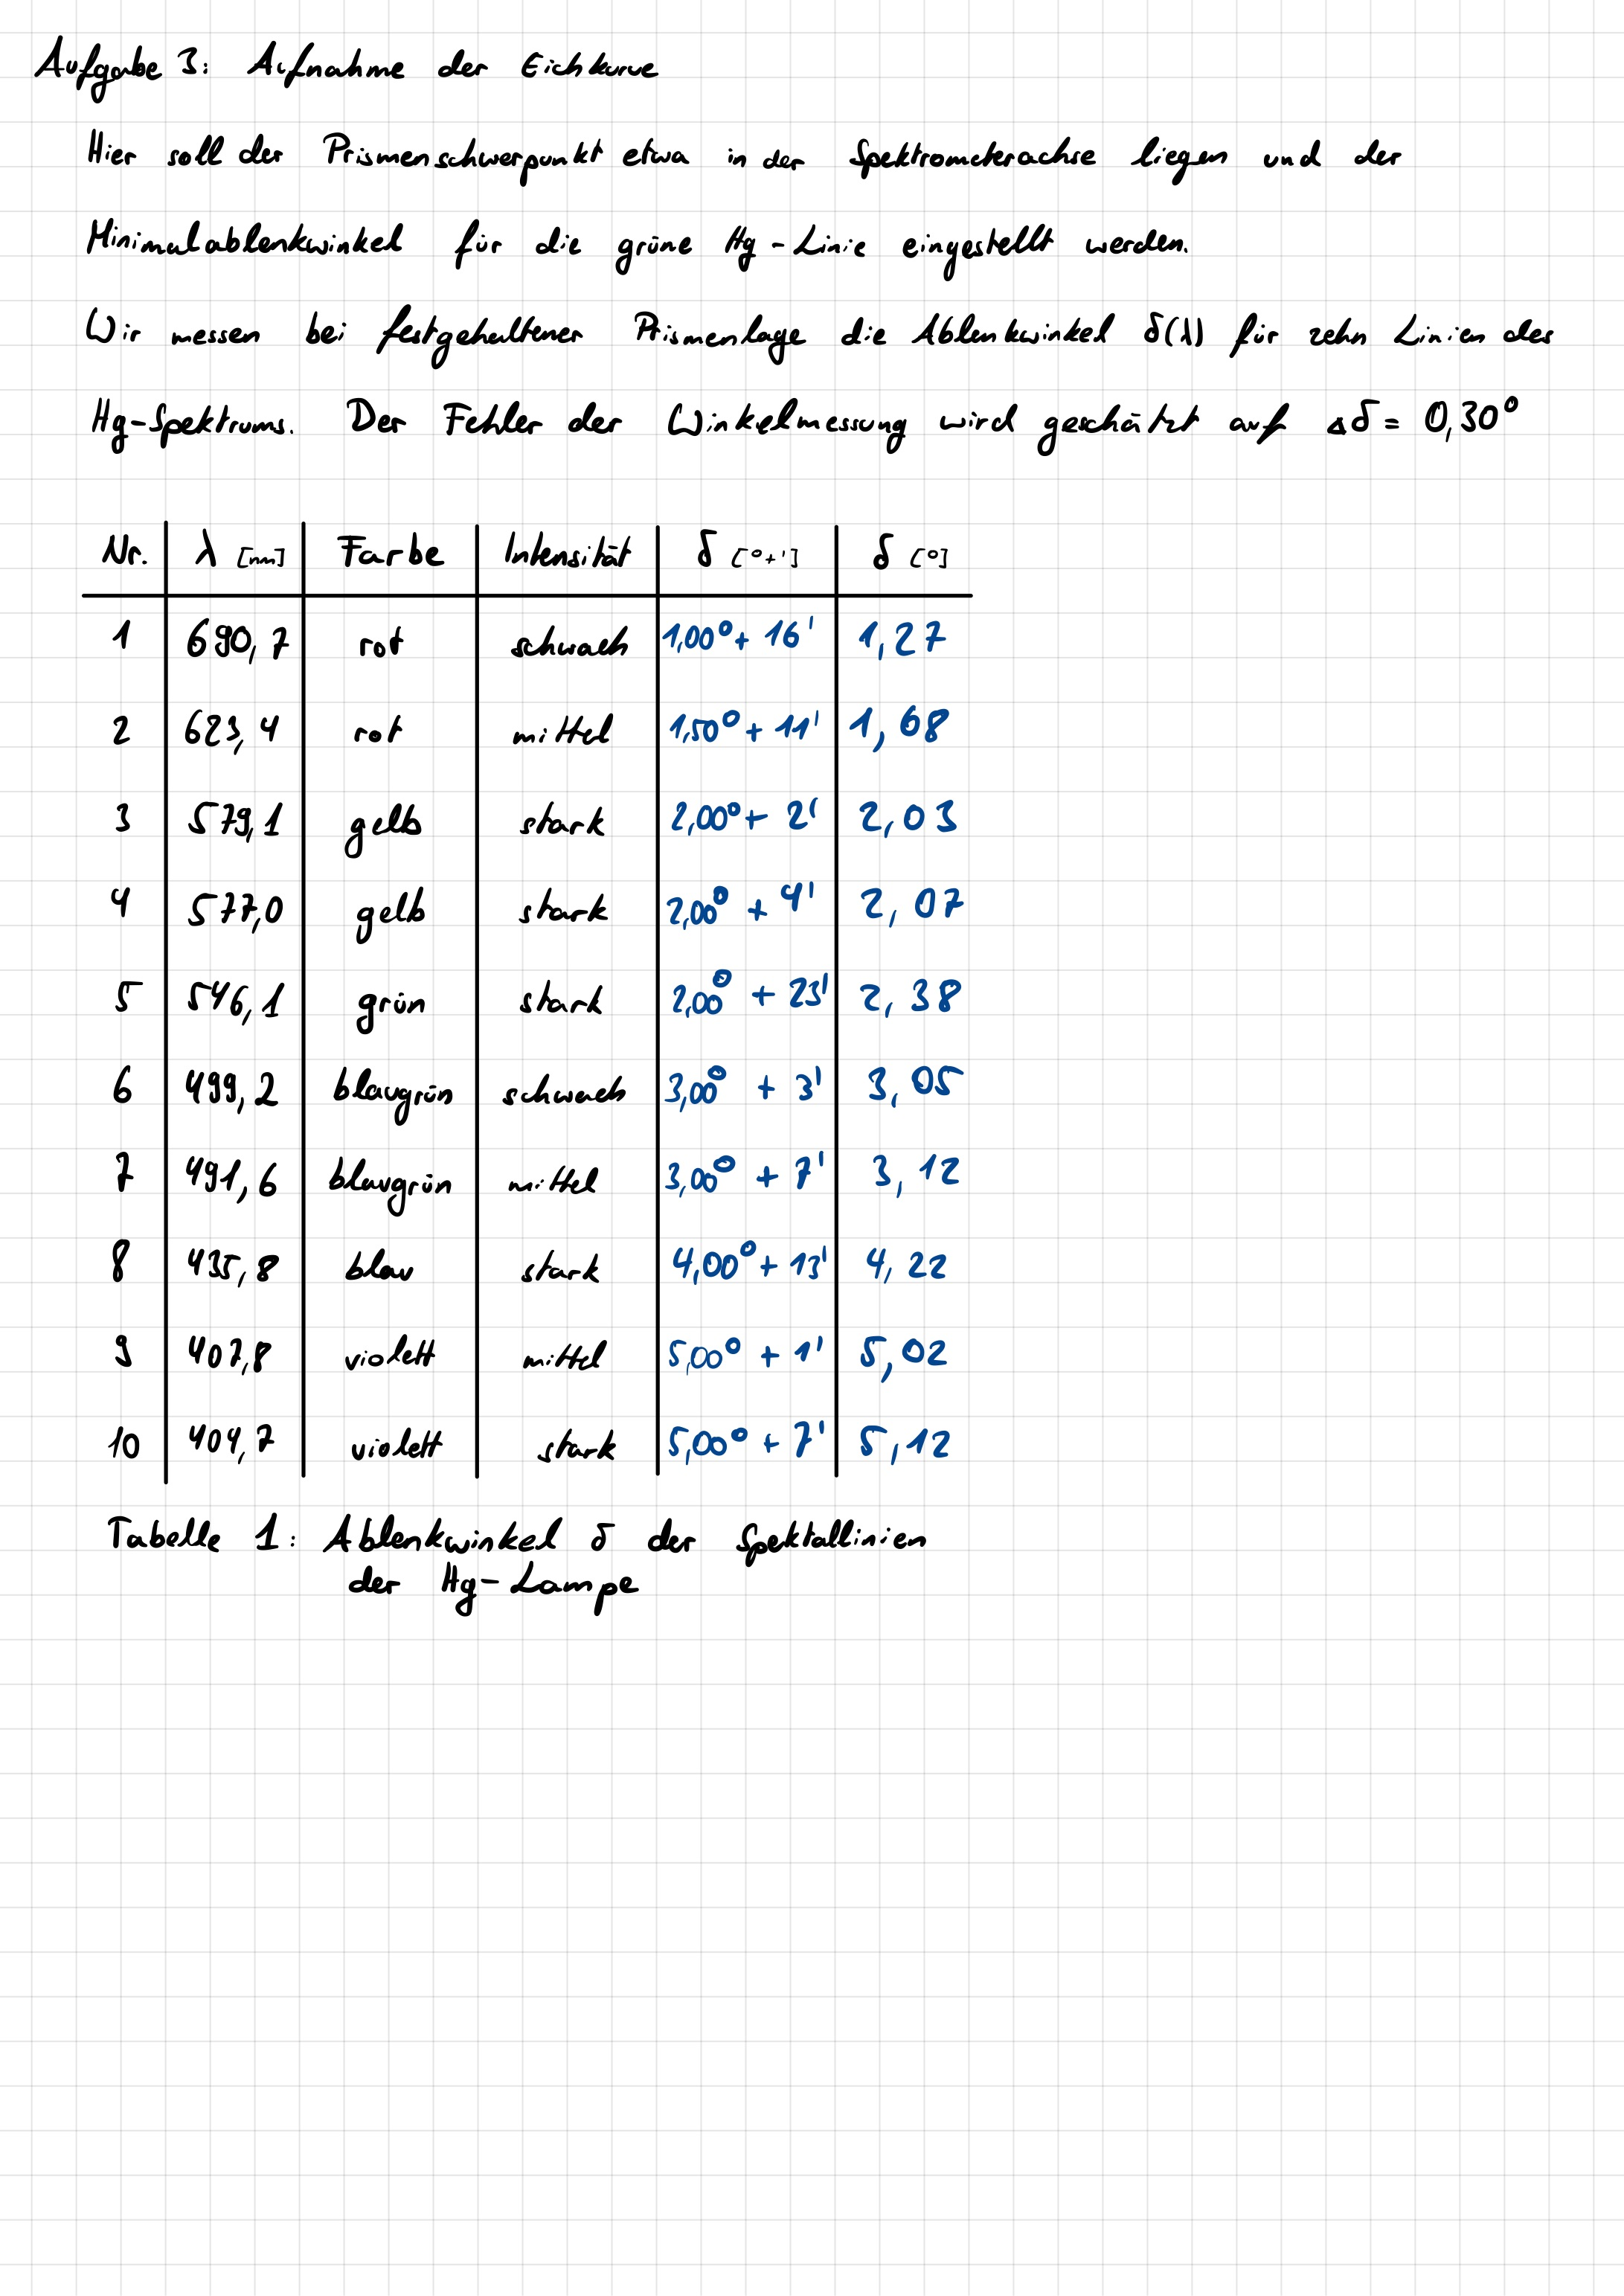
\includegraphics[width=\textwidth]{graphics/mess2.jpg}
\newpage
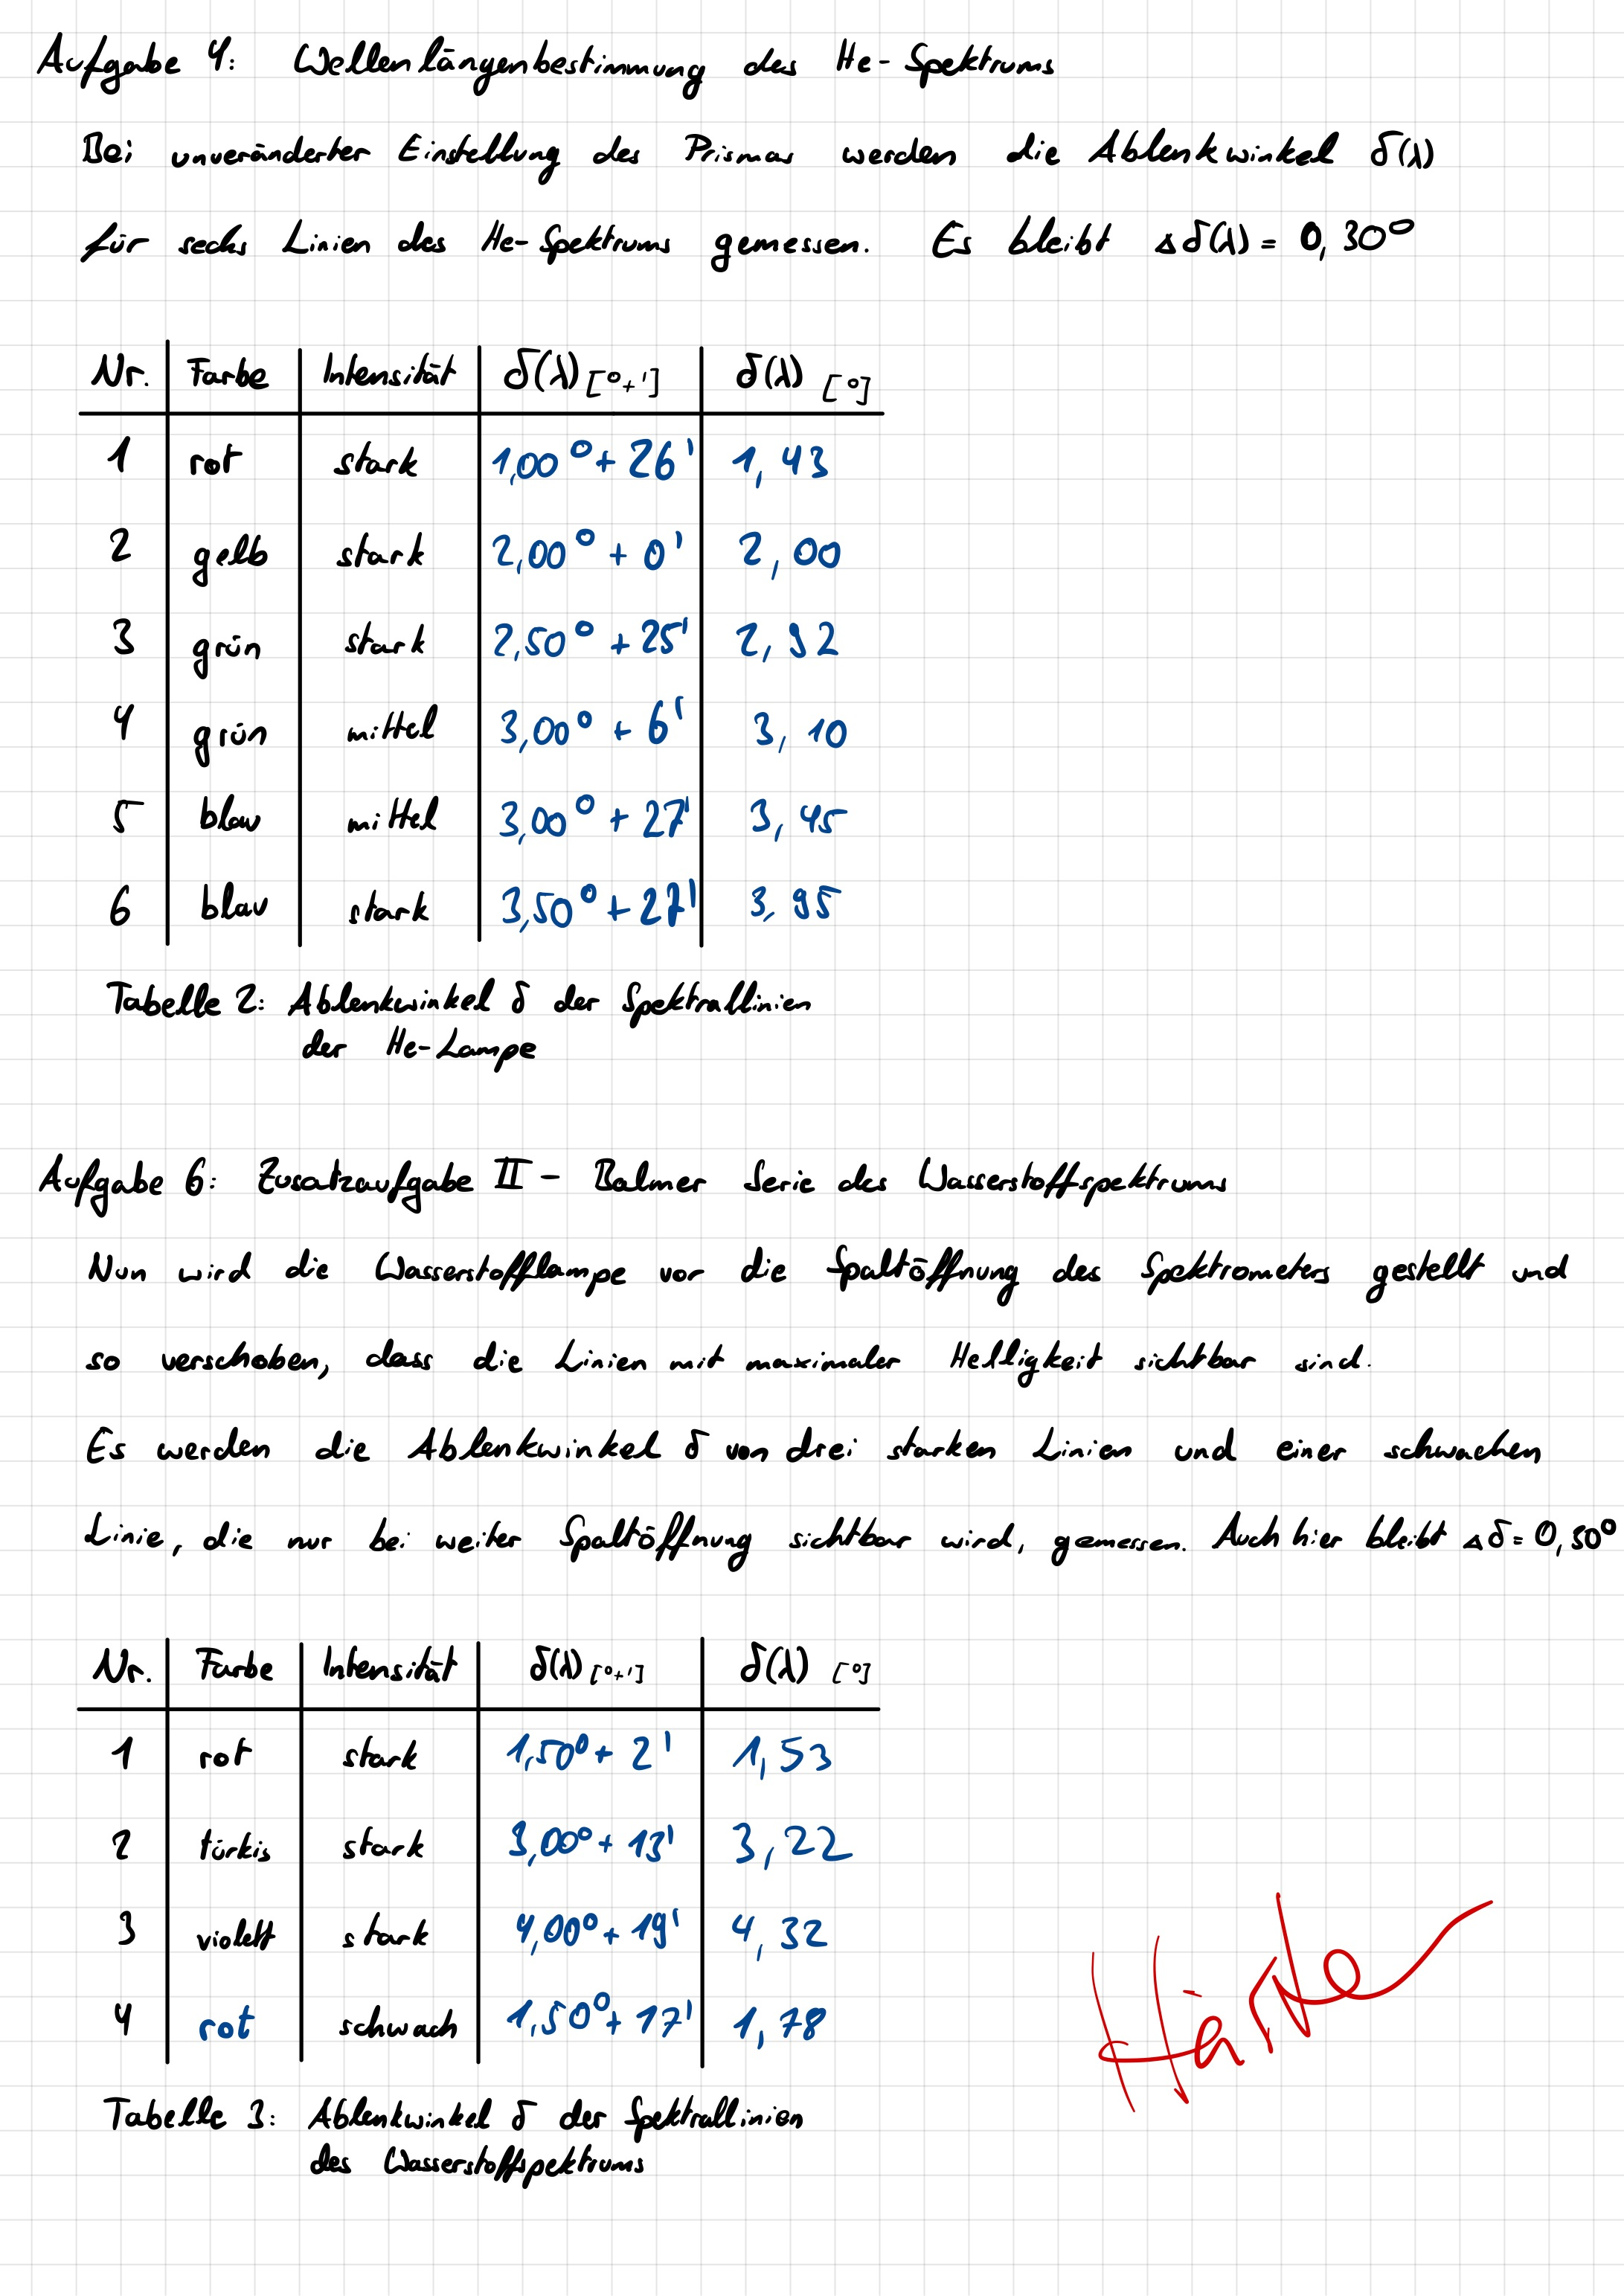
\includegraphics[width=\textwidth]{graphics/mess3.jpg}
\newpage

\addtocounter{table}{3}

%-------------------------AUSWERTUNG-------------------------
\section{Evaluation}

Auch hier müssen Tabellen und Grafiken eingefügt werden. Kopiere dafür den Code von oben.

%---------------PRÄSENTATION DER ENDERGEBNISSE---------------
\section{Presentation of final results}

blabla.

%---------------ZUSAMMENFASSUNG UND DISKUSSION---------------
\section{Summary and Discussion}

blabla.

\end{document}

